% ----------------------------------------------------------------
%       Speech Signal Processing Toolkit (SPTK): version 3.0
%                      SPTK Working Group
% 
%                Department of Computer Science
%                Nagoya Institute of Technology
%                             and
%   Interdisciplinary Graduate School of Science and Engineering
%                Tokyo Institute of Technology
%                   Copyright (c) 1984-2000
%                     All Rights Reserved.
% 
% Permission is hereby granted, free of charge, to use and
% distribute this software and its documentation without
% restriction, including without limitation the rights to use,
% copy, modify, merge, publish, distribute, sublicense, and/or
% sell copies of this work, and to permit persons to whom this
% work is furnished to do so, subject to the following conditions:
% 
%   1. The code must retain the above copyright notice, this list
%      of conditions and the following disclaimer.
% 
%   2. Any modifications must be clearly marked as such.
%                                                                        
% NAGOYA INSTITUTE OF TECHNOLOGY, TOKYO INSITITUTE OF TECHNOLOGY,
% SPTK WORKING GROUP, AND THE CONTRIBUTORS TO THIS WORK DISCLAIM
% ALL WARRANTIES WITH REGARD TO THIS SOFTWARE, INCLUDING ALL
% IMPLIED WARRANTIES OF MERCHANTABILITY AND FITNESS, IN NO EVENT
% SHALL NAGOYA INSTITUTE OF TECHNOLOGY, TOKYO INSITITUTE OF
% TECHNOLOGY, SPTK WORKING GROUP, NOR THE CONTRIBUTORS BE LIABLE
% FOR ANY SPECIAL, INDIRECT OR CONSEQUENTIAL DAMAGES OR ANY
% DAMAGES WHATSOEVER RESULTING FROM LOSS OF USE, DATA OR PROFITS,
% WHETHER IN AN ACTION OF CONTRACT, NEGLIGENCE OR OTHER TORTIOUS
% ACTION, ARISING OUT OF OR IN CONNECTION WITH THE USE OR
% PERFORMANCE OF THIS SOFTWARE.
% ----------------------------------------------------------------
%
\name{merge}{data merge}{data operation}

\begin{synopsis}
 \item[merge] [ --s $S$ ] [ --l $L_1$ ] [ --n $N_1$ ] [ --L $L_2$ ]
 [ --N $N_2$ ]
 \item[\ ~~~]  [ --o ] [ +{\em type} ] {\em file1} [ {\em infile} ] 
\end{synopsis}

\begin{qsection}{DESCRIPTION}
{\em merge} merges, on a frame-by-frame basis, data from {\em file1} 
into the data from {\em infile} (or standard input), 
sending the result to standard output, as described below.

\hspace{1cm}\includegraphics{fig/merge.eps}
\end{qsection}

\begin{options}
	\argm{s}{S}{insert point}{0}
	\argm{l}{L_1}{frame length of input data}{25}
	\argm{n}{N_1}{order of input data}{$L_1-1$}
	\argm{L}{L_2}{frame length of insert data}{10}
	\argm{N}{N_2}{order of insert data}{$L_2-1$}
	\argm{o}{}{overwrite mode}{FALSE}
	\argp{t}{input data format\\ 
		\begin{tabular}{llcll} \\[-1ex]
			c & char (1byte) & \quad &
			s & short (2bytes) \\
			i & int (4bytes) & \quad &
			l & long (4bytes) \\
			f & float (4bytes) & \quad &
			d & double (8bytes) \\
		\end{tabular}\\\hspace*{\fill}}{f}
\end{options}


\begin{qsection}{EXAMPLE}
The following example inserts blocks of 2 samples from {\em data.f2}
in short format into {\em data.f1}, also in short format,
the frame length of the file {\em data.f1} is 3, and the blocks
from {\em data.f2} will be inserted from the 3rd sample of
every frame.
The result is {\em data.merge}.
\begin{quote}
 \verb!merge -s 2 -l 3 -L 2 +s data.f2 < data.f1 > data.merge!
\end{quote}
For example, if the {\em data.f1} file is 
\[ 1,1,1,2,2,2,\cdots \], 
and the {\em data.f2} file is 
\[ 2,3,5,6,\cdots \]
then the output {\em data.merge} will be 
\[ 1,1,2,3,1,~ 2,2,5,6,2,\cdots \] 

The next example overwrites blocks of 2 samples from {\em data.f2}
in long format into {\em data.f1}, also in long format,
the frame length of the file {\em data.f1} is 4, and the blocks
from {\em data.f2} will be inserted from the 2nd sample of
every frame.
The result is {\em data.merge}.
\begin{quote}
 \verb!merge -s 2 -l 4 -L 2 +l -o data.f2 < data.f1 > data.merge!
\end{quote}
For example, if the {\em data.f1} file is 
\[ 1,1,1,1,2,2,2,2,\cdots \], 
and the {\em data.f2} file is 
\[ 3,4,5,6,\cdots \]
then the output {\em data.merge} will be 
\[  1,3,4,1,~ 2,5,6,2,\cdots \] 

\end{qsection}
